\chapter{Opis projektnog zadatka}

\section{Opis projektnog zadatka 'Štete javnih površina'}

\noindent Svakodnevno se suočavamo s brojnim problemima na javnim površinama i cestama u našim gradovima. Problemi kao što su vandalizam, oštećenje pločnika, udarne rupe na cestama, smeće i slično predstavljaju potencijalnu opasnost za građane te poprilično narušavaju kvalitetu njihovog svakodnevnog života.

\noindent Neadekvatna briga o oštećenjima i njihovoj sanaciji često ostavlja građane u vrlo nepovoljnoj situaciji kada iste žele prijaviti vlastima. Kako bi suzbili osjećaj nemoći građana i poboljšali kvalitetu života cjelokupne zajednice, potrebno je omogućiti adekvatnu prijavu oštećenja na javnim površinama.

\noindent Glavni je cilj ovog projekta razviti programsku podršku za stvaranje web aplikacije
CestaFix za dojavu oštećenja i drugih problema na cestama, parkovima, javnim ustanovama i ostalim javnim mjestima kako bi se olakšala dojava, kategorizacija te u konačnici rješenja prijavljenih problema. Ideja je omogućiti građanima da na što jednostavniji način prijavljuju oštećenja i probleme na javnim površinama i cestama svojih gradova te tako pomognu lokalnim vlastima da pravodobno reagiraju na nastale probleme.

\noindent S obzirom na velik broj javih ustanova i njihovih odjeljaka koji se bave različitim problemima, teško je pratiti tko je nadležan za koju vrstu problema i nad kojim područjem. Sustav bi automatski odredio nadležno tijelo prema kategoriji prijave i drugim parametrima te proslijedio prijavu na obradu. Ključno je da proces prijave bude jednostavan i brz.
\noindent Prilikom pokretanja sustava prikazuje se početna stranica na kojoj se nalazi karta s označenim lokacijama već podnesenih prijava raznovrsnih oštećenja javnih površina i navigacijski izbornik putem kojeg se pristupa registraciji/prijavi u sustav, podnošenju prijava, provjeri statusa već podnesenih prijava, često postavljanim pitanjima te informacijama o samoj aplikaciji.
\noindent Svakom neregistriranom korisniku omogućeno je kreiranje novog računa prilikom čega je potrebno unijeti:

\begin{packed_item}
	\item \textit{ime}
	\item \textit{prezime}
	\item \textit{lozinku}
	\item \textit{email adresu}
\end{packed_item}

\noindent Ako korisnik već ima postojeći račun, prilikom prijave u sustav unosi:

\begin{packed_item}
	\item \textit{email adresu}
	\item \textit{lozinku}
\end{packed_item}

\noindent Registrirani korisnik može pregledavati i mijenjati svoje osobne podatke i izbrisati svoj korisnički račun te postoji mogućnost naknadne dodjele prava službenika ili administratora stupanjem u kontakt naveden pri dnu stranice.

\noindent Također, postoji opcija anonimnog podnošenja prijave na temelju koje se status podnesene prijave prati putem jedinstvenog broja prijave bez iznošenja osobnih podataka i potrebe za registracijom odnosno prijavom.

Korisnik s pravom \underbar{službenika} ima mogućnost ažuriranja statusa prijava i pregled profila prijavitelja (ili jedinstvenog broja prijave u slučaju anonimnog prijavitelja) među kojima odabire relevantne prijave. Nakon što sustav proslijedi prijavu u nadležni gradski ured, službenik tog ureda može izabrati problem i krenuti raditi na njegovu rješenju.


\underbar{Administrator} sustava ima najveće ovlasti među koje pripada i pristup bazi s popisom registriranih korisnika i njihovim podacima te mogućnost brisanja korisnika kao i dodjeljivanje administratorskih prava i prava službenika drugim korisnicima.

\noindent Kako bi olakšala proces podnošenja prijave, aplikacija omogućuje građanima da brzo i precizno dokumentiraju probleme. Svaka prijava uključuje naziv problema, kratki opis, geografske koordinate problema, jedinstveni broj prijave te opcionalno fotografije kako bi se problem što bolje opisao.
\noindent Sustav također olakšava identifikaciju vremenski bliskih prijava na istoj lokaciji kako bi se građani mogli povezati na postojeće prijave sličnih problema, čime se smanjuje dupliciranje prijava i ubrzava proces njihovog rješavanja.
\noindent Podnesene prijave obrađuju određeni gradski uredi, a svaka promjena u statusu prijave vidljiva je prijavitelju i svim ostalim korisnicima.

\noindent Gradski uredi također imaju mogućnost objediniti nepovezane prijave na istoj lokaciji, što je vidljivo prijaviteljima.
\noindent Kako bi gradskim uredima olakšali razvrstavanje i obrađivanje prijava, sustav dopušta prijave za različite kategorije problema. Osnovne kategorije problema su:

\begin{packed_item}
	\item \textit{oštećenja na cesti}
	\item \textit{oštećenja na vodovodnoj infrastrukturi}
	\item \textit{oštećenja na zelenim površinama}
	\item \textit{oštećenja na elektroenergetskoj infrastrukturi}
\end{packed_item}

\noindent Sve podnesene prijave su javno dostupne i mogu se grupirati prema temi i lokaciji, što omogućuje građanima i vlastima da prate i analiziraju probleme u stvarnom vremenu.

\noindent Statistika o statusima prijava, poput vremena potrebnog za rješavanje problema, također se obrađuje u stvarnom vremenu kako bi poboljšala učinkovitost sustava i pomogla gradskim vlastima u praćenju učinkovitosti njihovih usluga.

\noindent Posebna je pozornost posvećena zaštiti svih osobnih podataka te osiguranju korisničkog iskustva koje će biti jednostavno i intuitivno, kako bi se potaknulo građane na aktivno sudjelovanje u poboljšanju svojih zajednica.

\noindent Skup korisnika koji bi mogao biti zainteresiran za ovu aplikaciju je vrlo širok. To uključuje građane koji žele prijaviti probleme na javnim površinama, lokalne gradove i njihove urede koji će obraditi prijave, službenike koji će nadzirati i rješavati prijave te administratore koji će upravljati sustavom i osigurati sigurnost podataka.

\noindent Jedan od primjera sličnog sustava koji se aktivno upotrebljava u Hrvatskoj je "Gradsko Oko". Projekt je pokrenut u kolovozu 2017. godine u svrhu prijave komunalnih problema na području grada Bjelovara, a od tad se proširio na još 11 gradova i općina te na prijavu problema na moru.

\begin{figure}[H]
	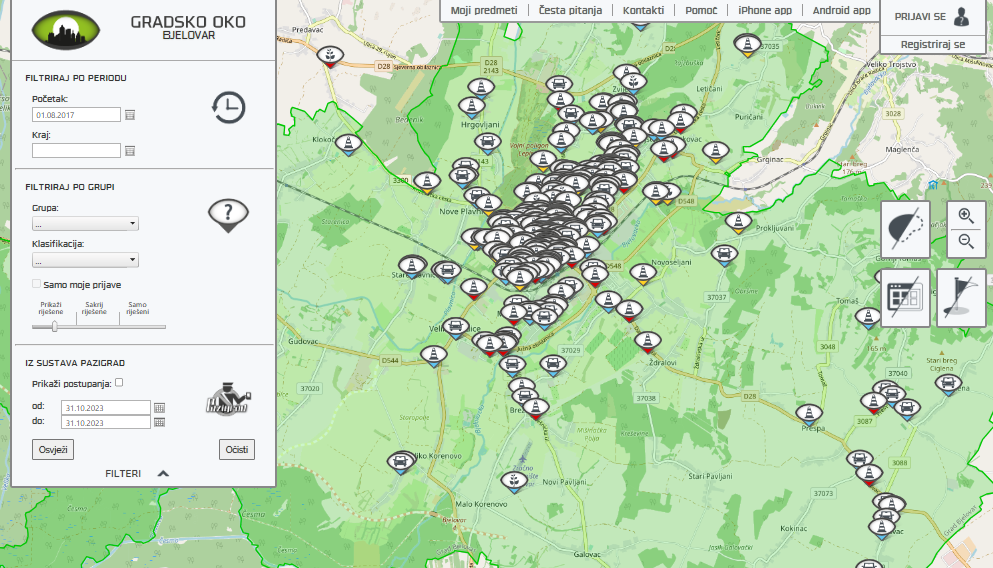
\includegraphics[scale=0.5]{slike/GradskoOko.png} %veličina slike u odnosu na originalnu datoteku i pozicija slike
	\centering
	\caption{Početna stranica sustava "Gradsko Oko"}
	\label{fig:GradskoOkoPrimjer}
\end{figure}

\newpage

\noindent Sustav “FixMyStreet” koji se koristi na području Ujedinjenog Kraljevstva također omogućava građanima da prijave probleme na javnim površinama i cestama u svojim lokalnim zajednicama kao i prikaz statističkih podataka o prijavljenim problemima, vremenskim okvirima za rješavanje i druge korisne informacije.

\begin{figure}[H]
	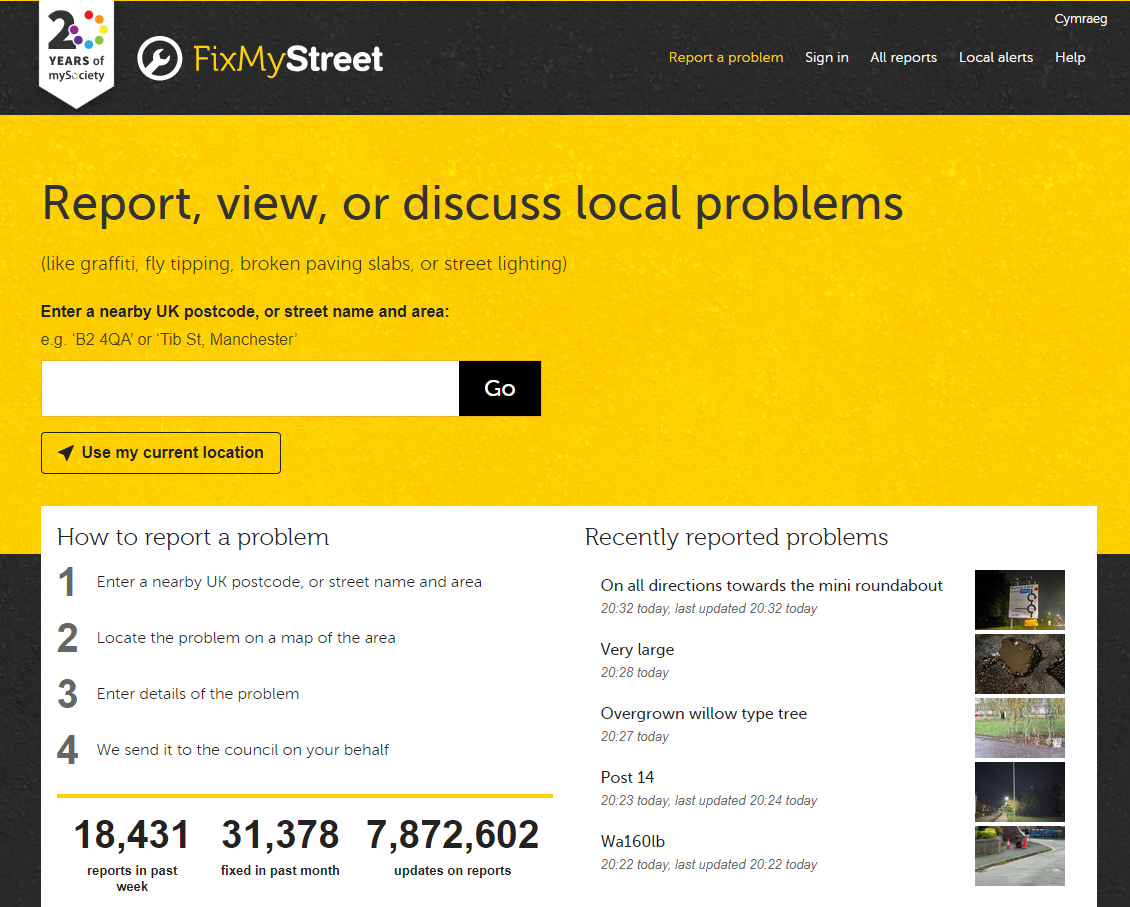
\includegraphics[scale=0.4]{slike/FixMyStreet.png} %veličina slike u odnosu na originalnu datoteku i pozicija slike
	\centering
	\caption{Početna stranica sustava "FixMyStreet"}
	\label{fig:FixMyStreet}
\end{figure}

\noindent Postojeća slična rješenja, kao što su "Gradsko Oko" i “FixMyStreet”, pružaju mogućnost prijave komunalnih problema, ali se razlikuju u nekoliko ključnih aspekata. Naša aplikacija ima određene značajke koje ju čine jedinstvenom, posebno u pogledu anonimnih prijava, statistike i praćenja rada gradskih ureda te povezivanja vremenski bliskih prijava.


\noindent Ova web aplikacija ima potencijal za prilagodbu i nadogradnje u budućnosti. Moguće nadogradnje uključuju integraciju s mobilnim aplikacijama kako bi se olakšao proces prijave, dodatne značajke za praćenje rada gradskih ureda, uvođenje sustava za nagrađivanje korisnika koji aktivno sudjeluju u rješavanju problema te proširenje na druge regije.

\eject






